\documentclass[12pt,letterpaper]{article}
\usepackage[utf8]{inputenc}
\usepackage{amsmath,amsthm,amsfonts,amssymb,amscd}
\usepackage[table]{xcolor}
\usepackage[margin=2.5cm]{geometry}
\usepackage{ragged2e}
\usepackage{graphicx}
\usepackage{multicol}
\usepackage{hyperref}
\usepackage{color}
\usepackage[brazil]{babel}
\newlength{\tabcont}
\setlength{\parindent}{0.0in}
\setlength{\parskip}{0.05in}

\begin{document}

	\begin{center}
		\Large \bf
		Relatório sobre MAC0214 - Atividade Curricular em Cultura e Extensão
	\end{center}
	
	\textbf{Nome}: Luís Felipe de Melo Costa Silva \\
	\textbf{Número USP}: 9297961
	
	\section*{Introdução}
	Para essa disciplina minha proposta era participar da organização do Encontro do BCC (e seu subevento Palestra do Ensino Médio) e do HackathonUSP. Além disso, prometi estar na Feira de Profissões da USP, como expositor do curso.
	
	\section{Encontro do BCC}
	O Encontro do BCC é um evento que acontece todos os anos desde 2009. Quem organiza são os próprios alunos do curso, e o público-alvo principal são os próprios alunos, além de quem se interessa por Computação de um modo geral. Neste dia, aconteceu entre os dias 21 e 25 de agosto.
	
	O Encontro chegou à sua IX edição esse ano. Tenho participado desde quando entrei, em 2015, então, já tenho uma noção do que tem que ser feito e de como o evento tem que parecer. 
	
	Basicamente, o que temos que preparar é:
	
	\begin{itemize}
		\begin{multicols}{2}
			\item Ciclo de Palestras;
			\item Conversa com os Professores do MAC;
			\item Ofícios;
			\item Divulgação;
			\item Patrocínios;
			\item Comida;
			\item Feira de Livros;
			\item Palestra do Ensino Médio.
		\end{multicols}
	\end{itemize}

	Abaixo, segue em detalhes o que é cada um desses itens e qual foi a minha contribuição em cada um deles.
	
	\subsection{Ciclo de Palestras}
	
	As palestras ocupam quase toda a semana do Encontro do BCC. Para esse ano, planejamos quatro dias de palestra, com quatro horas cada, logo, deveríamos ter no mínimo 16 palestrantes.
	
	Como todos os anos, liberamos um formulário para que os alunos sugerissem temas. Depois disso, filtramos essa lista (juntando temas semelhantes e removendo temas que não se encaixam na semana). A lista possui 17 temas, e pode ser vista na Figura 1.
	
	\begin{figure}
		\begin{center}
			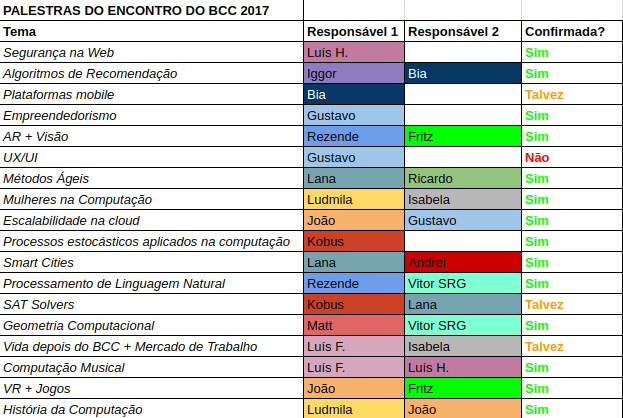
\includegraphics[scale=0.6]{palestras.png} 
			\caption{Tabela com os temas das palestras.}
		\end{center}
	\end{figure}

	Além desses temas, tínhamos alguns outros "na manga", caso necessário. Tudo isso para que não faltassem palestras na semana.
	
	Começamos a procura por palestrantes atribuindo duas palestras para cada pessoa e então, formando o máximo de duplas quanto possível. Decidimos assim para que a comunicação com os palestrantes fosse mais eficiente. 
	
	Como pode-se ver, fiquei com duas palestras inicialmente: \textit{Vida depois do BCC + Mercado de Trabalho} e \textit{Computação Musical}. Usando o texto que escrevi como modelo\cite{modelo_palestras}, comecei a mandar e-mails para possíveis palestrantes. 
	
	Para a palestra de \textit{Computação Musical}, contatei o professor Marcelo Queiroz do IME. Ele aceitou oferecer a palestra rapidamente, e por ser do instituto, seu horário era bem flexível.
	
	Contatei o ex-aluno Arthur Costa para dar a outra palestra, \textit{Vida depois do BCC + Mercado de Trabalho}, que aceitou no início mas teve que cancelar. Como estávamos no fim de julho, decidimos que essa palestra poderia não acontecer, já que as outras estavam bem encaminhadas (por isso o \textbf{{\color{orange} Talvez}} na tabela). No entanto, o Gustavo Silva, RD do curso, conseguiu que o Lucas Mendes, da Contratado.me desse a palestra (mais detalhes na subseção Patrocínios).
	
	Também relacionado a Patrocínios, consegui um palestrante para Algoritmos de Recomendação, o Matheus Cesário, da empresa Delivery Direto.
	
	No fim das contas, quase todas as palestras da tabela aconteceram, com exceção de \textit{UX/UI} e \textit{SAT Solvers}. Foram 15 palestras, já que a de Smart Cities teve duas horas. Os horários oficiais estão na Figura 2.
	
	\begin{figure}
		\begin{center}
			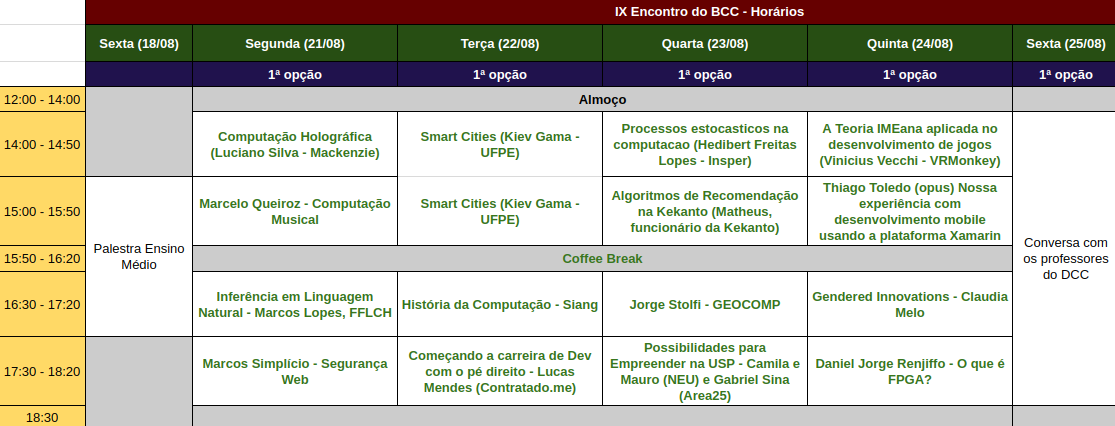
\includegraphics[scale=0.43]{horarios.png} 
			\caption{Tabela com os horários das palestras.}
		\end{center}
	\end{figure}

	Convidar os palestrantes e manter o contato com eles, elaborar um texto-modelo, fazer a tabela para controle das palestras e um \textit{Trello} para cuidar delas, gastei um total de \textbf{5 horas}. 
	
	\subsection{Conversa com os Professores e Entrega do PIPA}
	
	Para o último dia do evento, tradicionalmente realizamos a Conversa com os Professores do MAC. Não tem muito segredo, os professores e os alunos são convidados e nos reunimos em alguma sala que podemos fazer uma roda com as cadeiras. Acreditamos que isso promove uma aproximação entre os docentes e os discentes.
	
	Este ano, houve a Entrega do PIPA, no mesmo dia. Quem faria o discurso seria o RD do curso, mas ele não pôde estar presente, então eu o fiz. 
	
	Com a minha preparação, a apresentação e a Conversa com os Professores, dediquei neste dia \textbf{3 horas}.
	
	\subsection{Ofícios}
	
	Os ofícios são a parte burocrática da organização. Toda a comunicação com o IME é feita a partir deles. Autorização para realizar o evento, reserva de auditório, autorização para feira de livros e verba para o evento são conseguidos via ofícios, por exemplo.
	
	Minha contribuição com eles foi quase nula, já que estão todos prontos de anos anteriores e eu não fiquei responsável por entregar nenhum deles.
	
	A única coisa relacionada a isso que estive presente foi quando um deles foi mal interpretado. Todos os palestrantes são voluntários, mas o pedido de verba feito pela CPG incluía além, de passagem e hospedagem, um bônus pela realização da palestra. Isso foi resolvido rapidamente, e sem precisar de um novo ofício. Nesse mesmo dia, auxiliei em problemas relacionados à feira de livros (esclarecemos que os livros seriam guardados no anexo da sala B7).
	
	Com isso, apenas \textbf{30 minutos} foram gastos com assuntos relacionados a ofícios.
	
	\subsection{Divulgação}
	
	A Divulgação do evento é uma parte muito importante, porque, sem ela, as pessoas não viriam ao evento. A divulgação é feita de diversas maneiras:
	
	\begin{itemize}
		\item Site próprio
		\item Sites da USP e painéis eletrônicos pelo campus
		\item \textit{Página no Facebook}
		\item E-mails em listas do IME
		\item Cartazes colados na USP e no IME.
	\end{itemize}

	Não produzi nenhum dos citados acima. Fica aqui um reconhecimento do trabalho dos alunos do primeiro ano.Um deles fez quase todo o site e um outro conseguiu o cartaz. 
	
	Saímos para colar os cartazes pela USP, em diversas localizações\cite{cartazes}. Foram \textbf{2 horas} colando cartazes. 
	
	\subsection{Patrocínios}
	
	\subsection{Comida}
	
	\subsection{Palestra do Ensino Médio}
	
	\subsection{A semana}
	
	\section{HackathonUSP}
	
	\subsection{Preparação}
	
	\subsection{O evento}
	
	\section{Feira de Profissões}
	
	\section*{Considerações finais}
	
	\subsection*{Encontro do BCC}
	
	\subsection*{HackathonUSP}
	
	\subsection*{Feira de Profissões}
	
	\bibliographystyle{plain}
	
	\begin{thebibliography}{1}
		
		\bibitem{modelo_palestras}
		Arquivo com modelo de texto para convite de palestrantes.
		\newblock Disponível em \texttt{https://lsflp.github.io/MAC0214/encontro/palestras/palestras.pdf}.
		\newblock Consultado em 15 de novembro de 2017.
		
		\bibitem{cartazes}
		Divulgação por Cartazes do Encontro do BCC.
		\newblock Disponível em \texttt{https://lsflp.github.io/MAC0214/encontro/cartazes/cartazes.html}.
		\newblock Consultado em 15 de novembro de 2017.
		
		
		\bibitem{maragos89:_patter}
		P.~Maragos.
		\newblock Pattern spectrum and multiscale shape representation.
		\newblock {\em IEEE Trans. Patt. Anal. Mach. Intell.}, 11:701--715, 1989.
		
		\bibitem{Meijster:Wilkinson:PAMI}
		A.~Meijster and M.~H.~F. Wilkinson.
		\newblock A comparison of algorithms for connected set openings and closings.
		\newblock {\em IEEE Trans. Patt. Anal. Mach. Intell.}, 24(4):484--494, 2002.
		
		\bibitem{Nacken:thesis}
		P.~F.~M. Nacken.
		\newblock {\em Image Analysis Methods Based on Hierarchies of Graphs and
			Multi-Scale Mathematical Morphology}.
		\newblock PhD thesis, University of Amsterdam, Amsterdam, The Netherlands,
		1994.
		
	\end{thebibliography}
	
			 
\end{document}